\begin{tikzpicture}
    \draw[thick, rounded corners = 3pt] (0, 0) rectangle (3, -3);
    \draw[fill = orange!8, rounded corners = 3pt] (0.5, -0.5) rectangle (2.5, -2.5);
    \node at (-0.3, -1.5) {$X$};
    \node at (1.5, 0.3) {$Y$};

    \draw[red, dashed] (0.6, 0.3) -- (0.6, -0.5);
    \draw[red, line width = 2pt] (0.6, -0.5) -- (0.6, -2.5);
    \draw[red, dashed] (0.6, -2.5) -- (0.6, -3.3);

    \pause
    \only<3->{
        \draw[fill = green!50, rounded corners = 3pt, opacity = 0.3] (0.3, -0.3) rectangle (1.4, -1.8);
        \draw[fill = blue!50, rounded corners = 3pt, opacity = 0.3] (0.4, -1.5) rectangle (1, -2.2);
        \draw[fill = cyan!50, rounded corners = 3pt, opacity = 0.3] (0.2, -2.1) rectangle (0.8, -2.6);
    }

    \pause
    \only<4->{
        \draw[fill = black!80] (1.4, -0.5) {[rounded corners = 3pt] -- (2.5, -0.5)} -- (2.5, -1.8) -- (1.4, -1.8) -- cycle;
    }

    \pause
    \only<5->{
        \draw[red, dashed] (1.5, 0.3) -- (1.5, -0.5);
        \draw[red, line width = 2pt] (1.5, -0.5) -- (1.5, -1.8);
        \draw[red, dashed] (1.5, -1.8) -- (1.5, -3.3);
    }

    \pause
    \only<6->{
        \draw[fill = white!50, rounded corners = 3pt, opacity = 0.3] (1.4, -0.4) rectangle (1.8, -0.6);
        \draw[fill = white!50, rounded corners = 3pt, opacity = 0.3] (1.4, -0.6) rectangle (1.8, -1);
        \draw[fill = white!50, rounded corners = 3pt, opacity = 0.3] (1.4, -0.9) rectangle (1.7, -2);
        
    }
        

    \onslide<1->
\end{tikzpicture}
